\documentclass[9pt]{beamer}
\useoutertheme{split} 
\usecolortheme{beaver} %Color theme
\useinnertheme{rounded} %Places bullets and numbers in a rectangular background.

\usepackage{graphicx}
\usepackage{tikz}
\usetikzlibrary{backgrounds}
\usepackage{amssymb}

\tikzstyle{cover}=[rectangle,inner sep=1pt,outer sep=0pt]
\tikzstyle{nb}=[fill=red]
\tikzstyle{lv}=[fill=black!80]
\tikzstyle{bd}=[fill=black]
\tikzstyle{wl}=[fill=white]

\begin{document}
%%information
\title{Operating Signal by Amplifier}
\author{Sung Han Ro}
\institute{KAIST}
\date{Physical Mathematics I Conference\\
12 December 2009}
%%title page
\begin{frame}
\titlepage
\end{frame}
%%contents
\begin{frame}{Outline}
\tableofcontents
\end{frame}

%%Introduction
\section{Introduction}

\subsection{Signal}
%%frame1
\begin{frame}{Structure of Operating Signal}
Operating signal is essential technique of modern computing system. Nice signal and operating signals are required to have several properties.

\begin{itemize}
\onslide<2->{\item \alert{First of all, What is Signal?}} 

\begin{itemize}
\onslide<3-> {
\item Signal is any time varying or spatial varying quantity
\item Signal can carry information
}
\end{itemize}

\onslide<4->{\item \alert{Which quantity is good for Signal?}}

\begin{itemize}
\onslide<5->{Voltage!}
\end{itemize}

\onslide<6->{\item \alert{Signal Operation}}
\end{itemize}
\end{frame}

\subsection{Operation}
%%frame2
\begin{frame}{Objects used in operation}
%%%figure
\begin{center}
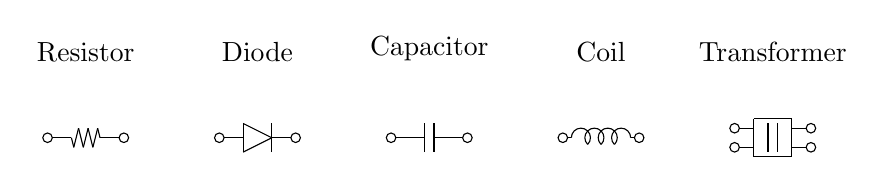
\begin{tikzpicture} [x=0.01\textwidth, y=0.01\textwidth]
%%position
\path (0,-3);
%%resistor
%%body
\draw[-] [bd] (1,0)--(3,0);
\draw[-] [bd] (3,0)--(3.25,-1);
\draw[-] [bd] (3.25,-1)--(3.75,1);
\draw[-] [bd] (3.75,1)--(4.25,-1);
\draw[-] [bd] (4.25,-1)--(4.75,1);
\draw[-] [bd] (4.75,1)--(5.25,-1);
\draw[-] [bd] (5.25,-1)--(5.75,1);
\draw[-] [bd] (5.75,1)--(6,0);
\draw[-] [bd] (6,0)--(8,0);
%%node
\draw (0.5,0) circle (0.5);
\draw (8.5,0) circle (0.5);
%%name
\path (4.5,7) node[above]{Resistor};
%%diode
%%body
\draw[-] [bd] (19,0)--(21,0);
\draw[-] [bd] (21,1.5)--(21,-1.5);
\draw[-] [bd] (21,1.5)--(24,0);
\draw[-] [bd] (21,-1.5)--(24,0);
\draw[-] [bd] (24,1.5)--(24,-1.5);
\draw[-] [bd] (24,0)--(26,0);
%%node
\draw (18.5,0) circle (0.5);
\draw (26.5,0) circle (0.5);
%%name
\path (22.5,7) node[above] {Diode};
%%capacitor
%%body
\draw[-] [bd] (37,0) -- (40,0);
\draw[-] [bd] (40,1.5)--(40,-1.5);
\draw[-] [bd] (41,1.5)--(41,-1.5);
\draw[-] [bd] (41,0)--(44,0);
%%node
\draw (36.5,0) circle(0.5);
\draw (44.5,0) circle(0.5);
%%name
\path (40.5,7) node[above] {Capacitor};
%%coil
%%body
\draw (55,0)--(55.4,0);
\draw (61.6,0)--(62,0);
%
\draw (57.1,-0.7) arc (-45:180:1);
\draw (57.1,-0.7) arc (225:-45:1);
\draw (58.5,-0.7) arc (225:-45:1);
\draw (59.9,-0.7) arc (225:0:1);
%%node
\draw (54.5,0) circle (0.5);
\draw (62.5,0) circle (0.5);
%%name
\path (58.5,7) node[above] {Coil};
%%transformer
%% body
\draw (74.5,2) -- (78.5,2) -- (78.5,-2) --(74.5,-2) -- (74.5,2);
\draw (76,1.5) -- (76,-1.5);
\draw (77,1.5) -- (77,-1.5);
%%wire
\draw (73,1) -- (74.5,1);
\draw (73,-1) -- +(1.5,0);
\draw (78.5,1) -- +(1.5,0);
\draw (78.5,-1) -- +(1.5,0);
%%node
\draw (72.5,1) circle (0.5);
\draw (72.5,-1) circle (0.5);
\draw (80.5,1) circle (0.5);
\draw (80.5,-1) circle (0.5);
%%name
\path (76.5,7) node[above] {Transformer};
\end{tikzpicture}
\end{center}

\begin{itemize}
\color<2->{gray}{
\item \alert<1>{Resistor }
\begin{equation}
I = \frac{V}{R}
\end{equation}
\item \alert<1>{Diode}
\begin{equation}
I = I_0 e^{kV}
\end{equation}
\item \alert<1>{Capacitor}
\begin{equation}
I = C \frac{d}{dt}V
\end{equation}
\item \alert<1>{Coil}
\begin{equation}
I = -\frac{1}{L} \int V dt
\end{equation}
}
\item \alert<1->{Transformer}
\begin{equation}
\alert<2->{V_{out} = \frac{N_{in}}{N_{out}} V_{in}}
\end{equation}
\end{itemize}
\end{frame}

%%frame3
\begin{frame}{Structure of Operating Signal}
Operating signal is essential technique of modern computing system. Nice signal and operating signals are required to have several properties.

\begin{itemize}
\onslide<1->{\item \alert{First of all, What is Signal?}} 

\begin{itemize}
\onslide<1-> {
\item Signal is any time varying or spatial varying quantity
\item Signal can carry information
}
\end{itemize}

\onslide<1->{\item \alert{Which quantity is \alert{good} for Signal?}}

\begin{itemize}
\onslide<1->{Voltage!}
\end{itemize}

\item \alert{Signal Operation}
\onslide<2->{

\begin{itemize}
\item Input and output signal have to be same type
\item Operating method should cover general cases
\end{itemize}
}
\end{itemize}
\onslide<3->{
\begin{center}
\alert{How??}
\end{center}
}
\end{frame}

%%Signal Operation by Amplifier
\section{Signal Operation by Amplifier}
%%
\subsection{Operational Amplifier}
%%frame4
\begin{frame}{Operational amplifier}
As a base of signal operation, Operational amplifier is widely used 
%%figure
\begin{center}
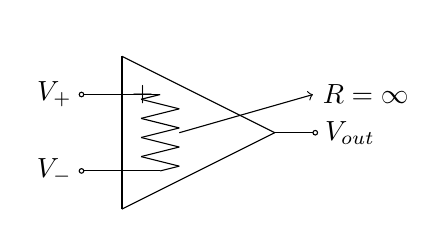
\begin{tikzpicture}[x=0.02\textwidth, y=0.02\textwidth]
%%positioning
\path (0,5.5)--(0,5);
%%body
\draw[-] [bd] (0,-4)--(0,4);
\draw[-] [bd] (0,4)--(8,0);
\draw[-] [bd] (0,-4)--(8,0);
%%wire
\draw[-] [bd] (-2,2)--(0,2); 
\onslide<1> {\path (0,2) node[right]{+};} 
\draw[-] [bd] (-2,-2)--(0,-2); 
\onslide<1> {\draw (0.75,-2) -- (1.65,-2) ;} 
\draw[-] [bd] (8,0)--(10,0);
%%node
\draw (-2.12,-2) circle (0.12) node[left] {$V_-$};
\draw (-2.12,2) circle (0.12) node[left]{$V_+$};
\draw (10.12,0) circle (0.12) node[right]{$V_{out}$};
%%resistor
\onslide<2->{
\draw (0,2)--(2,2);
\draw (0,-2)--(2,-2);

\draw (2,2)--(1,1.75);
\draw (1,1.75)--(3,1.25);
\draw (3,1.25)--(1,0.75);
\draw (1,0.75)--(3,0.25);
\draw (3,0.25)--(1,-0.25);
\draw (1,-0.25)--(3,-0.75);
\draw (3,-0.75)--(1,-1.25);
\draw (1,-1.25)--(3,-1.75);
\draw (3,-1.75)--(2,-2);
\draw [->] (3,0)--(10,2) node[right]{$R = \infty$};
}
\end{tikzpicture}
\end{center}
%%equation of amp

\onslide<3->{
\begin{equation}
V_{out} = \lim _{G \rightarrow \infty} G \left( V_+ - V_-  \right) \label{amp}
\end{equation}
}
%%describtion
\begin{itemize}
\onslide<4->{
\item OP-amp amplify input voltage with Gain $G$
\item In ideal case, $G$ is infinitely large number
}
\end{itemize}
\end{frame}
%%
\subsection{Simple Examples}
%%frame5
\begin{frame}{Simple OP-amp circuit : Inverting amplifier}
%%
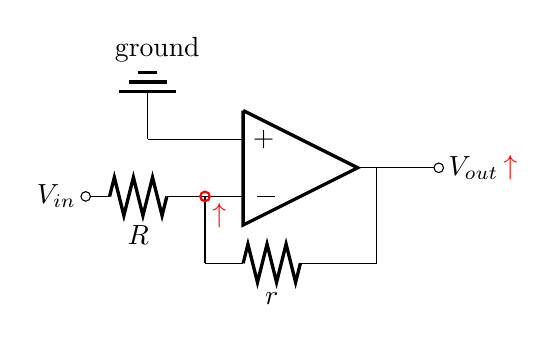
\begin{tikzpicture}[x=0.01\textwidth, y=0.01\textwidth]
\draw [very thick](0,6) -- (12,0) -- (0,-6) -- (0,6);
\draw (-10,3) -- (0,3) node[right]{+};
\draw (-8,-3) -- (0,-3);
\draw (1.5,-3) -- (3.3,-3);
\draw (12,0) -- (20,0);
\draw (20.5,0) circle (0.5) node[right]{$V_{out}$};
%%resistor
\draw [very thick](-8,-3) -- (-8.5, -5) -- (-9.5,-1) -- (-10.5,-5) -- (-11.5,-1) -- (-12.5,-5) -- (-13.5,-1) -- (-14,-3);
\path (-11,-5) node[below] {$R$};
%%%
\draw (-14,-3) -- (-16,-3);
\draw (-16.5,-3) circle (0.5) node[left]{$V_{in}$};
\draw (-4,-3) -- (-4,-10);
\draw (-4,-10) -- (0,-10);
\draw [very thick](0,-10) -- (0.5, -8) -- (1.5, -12) -- (2.5, -8) -- (3.5,-12) -- (4.5,-8) -- (5.5,-12) -- (6,-10);
\path (3,-12) node[below]{$r$};
%%%
\draw (6,-10) -- (14,-10) -- (14,0);
%%ground
\draw (-10,3) -- (-10, 8);
\draw [very thick](-13,8) -- (-7,8);
\draw [very thick](-12,9) -- (-8,9);
\draw [very thick](-11,10) -- (-9,10) node[above]{ground}; 
%%control
\onslide<3->{\path[red] (28,0) node{$\uparrow$};}
\onslide<4->{
\path[red] (-2.5,-5) node{$\uparrow$};
\draw[thick][red] (-4,-3) circle(0.5);
}
\end{tikzpicture}

\begin{itemize}
\onslide<2->{
\item \alert{$V_{out}$ and $V_{-}$ connected} 
}
\begin{itemize}
\onslide<5->{
\item $V_{out} \rightarrow$ Finite
}
\onslide<6->{
\item Finite $V_{out} \rightarrow V_- = V_+ = 0$ \onslide<6>{[Remind \alert{$\lim _{G \rightarrow \infty} G(V_+ - V_-)$}]}
}
\end{itemize}
\onslide<7->{
\item \alert{$V_{in} \rightarrow V_{out}$ current}
\begin{itemize}
\item $i = V_{in}/R = -V_{out}/r$ 
\end{itemize}
}
\end{itemize}

\onslide<8->{
\begin{equation}
V_{out} = -\frac{r}{R} V_{in}
\end{equation}
}
\end{frame}

%%General Rule
\subsection{General Rule}
\begin{frame}{Principle of OP-amp operation}
%%%
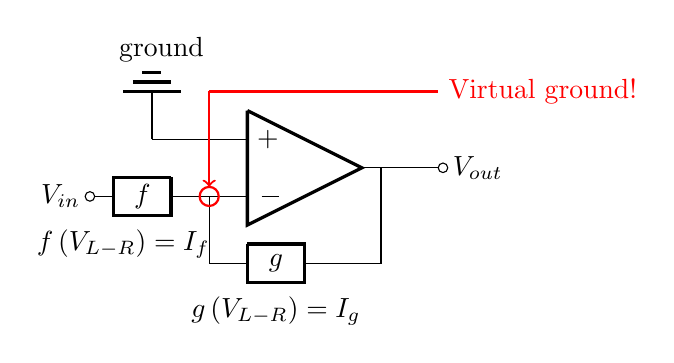
\begin{tikzpicture}[x=0.01\textwidth, y=0.01\textwidth]
\draw [very thick](0,6) -- (12,0) -- (0,-6) -- (0,6);
\draw (-10,3) -- (0,3) node[right]{+};
\draw (-8,-3) -- (0,-3);
\draw (1.5,-3) -- (3.3,-3);
\draw (12,0) -- (20,0);
\draw (20.5,0) circle (0.5) node[right]{$V_{out}$};
%%ground
\draw (-10,3) -- (-10, 8);
\draw [very thick](-13,8) -- (-7,8);
\draw [very thick](-12,9) -- (-8,9);
\draw [very thick](-11,10) -- (-9,10) node[above]{ground}; 
%%object
\draw [very thick](-8,-1) -- (-8,-5) -- (-14,-5) -- (-14,-1) -- (-8,-1);
\draw (-14,-3) -- (-16,-3);
\draw (-16.5,-3) circle (0.5) node[left]{$V_{in}$};

\draw (-4,-3) -- (-4,-10) -- (0,-10);
\draw [very thick](0,-8) -- (0,-12) -- (6,-12) -- (6,-8) -- (0,-8);

\draw (6,-10) -- (14,-10) -- (14,0);
\path (3,-10) node{$g$};
\path (-11,-3) node{$f$};

\onslide<2->{\path (-13,-8) node{$f \left(V_{L-R} \right) = I_{f}$};}
\onslide<3->{\path (3,-15) node{$g \left( V_{L-R} \right) = I_{g}$};}
\onslide<5->{
\draw [thick] [red] (-4,-3) circle (1);
\draw [->][thick] [red] (-4,8) -- (-4,-2);
\draw [thick][red] (-4,8)--(20,8) node[right]{Virtual ground!};
}
\end{tikzpicture}

\begin{itemize}
\onslide<4->{
\item \alert{Negative feedback}
\begin{itemize}
\item $V_{out}$ fixed on equilibrium value
\item Finite $V_{out} \rightarrow V_- = V_+ = 0$
\end{itemize}
}
\onslide<6->{\item  \alert{$V \rightarrow I \rightarrow V$}}
\begin{itemize}
\onslide<7->{\item Current fixed at $I_{in} = f \left( V_{in} \right)$}
\onslide<8->{\item Current also satisfy $I_{in} = g \left( -V_{out} \right)$}
\end{itemize}

\end{itemize}
\onslide<9->{
\begin{equation}
\alert{V_{out} = - g^{-1} \left[ f \left( V_{in}\right) \right]}
\end{equation}
}
\end{frame}

%%Applications
\section{Applications}
\subsection{Single - Signal Operator}
\begin{frame}{Exponential operator}
%%%%
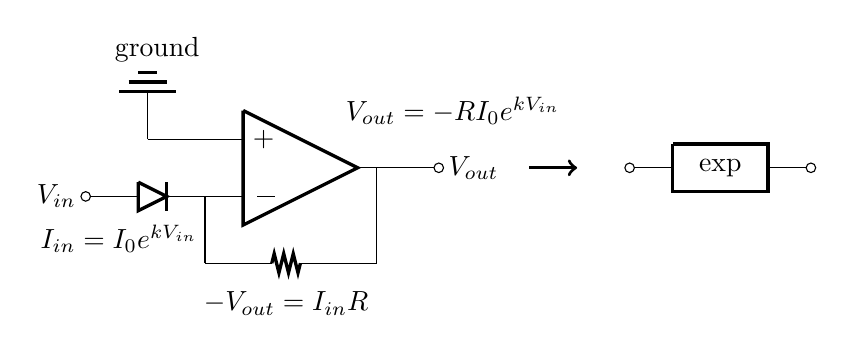
\begin{tikzpicture}[x=0.01\textwidth, y=0.01\textwidth]
\draw [very thick](0,6) -- (12,0) -- (0,-6) -- (0,6);
\draw (-10,3) -- (0,3) node[right]{+};
\draw (-8,-3) -- (0,-3);
\draw (1.5,-3) -- (3.3,-3);
\draw (12,0) -- (20,0);
\draw (20.5,0) circle (0.5) node[right]{$V_{out}$};
\draw (-11,-3) -- (-16,-3);
\draw (-16.5,-3) circle (0.5) node[left]{$V_{in}$};
\draw (-4,-3) -- (-4,-10);
\draw (-4,-10) -- (3,-10);
\draw (6,-10) -- (14,-10) -- (14,0);

%%resistor
\draw [very thick](-11,-1.5) -- (-11,-4.5) -- (-8,-3) -- (-11,-1.5);
\draw [very thick](-8,-1.5) -- (-8,-4.5);
%%%
\onslide<2->{
\path (-13,-5) node[below] {$I_{in} = I_0 e^{k V_{in}}$};
}
%%%
\draw [very thick](3,-10) -- (3.25, -9) -- (3.75, -11) -- (4.25, -9) -- (4.75,-11) -- (5.25,-9) -- (5.75,-11) -- (6,-10);
%%%%
\onslide<3->{
\path (4.5,-12) node[below]{$- V_{out} = I_{in} R$};
}
%%%
%%ground
\draw (-10,3) -- (-10, 8);
\draw [very thick](-13,8) -- (-7,8);
\draw [very thick](-12,9) -- (-8,9);
\draw [very thick](-11,10) -- (-9,10) node[above]{ground}; 
%%%result
\onslide<4->{
\path (22,6) node{\alert{$V_{out} = - RI_0  e^{k V_{in}}$}};
}
%%abstraction
\onslide<5->{
\draw [->][very thick] (30,0) -- (35,0);
\draw (40.5,0) circle (0.5);
\draw (41,0) -- (45,0);
\draw [very thick](45,2.5)--(45,-2.5)--(55,-2.5)--(55,2.5)--(45,2.5);
\draw (55,0) -- (59,0);
\draw (59.5,0) circle (0.5);
\path (50,0) node{exp};
}
\end{tikzpicture}
%%%%%
\end{frame}

%%%%
\begin{frame}{Logarithmic operator}
%%%%
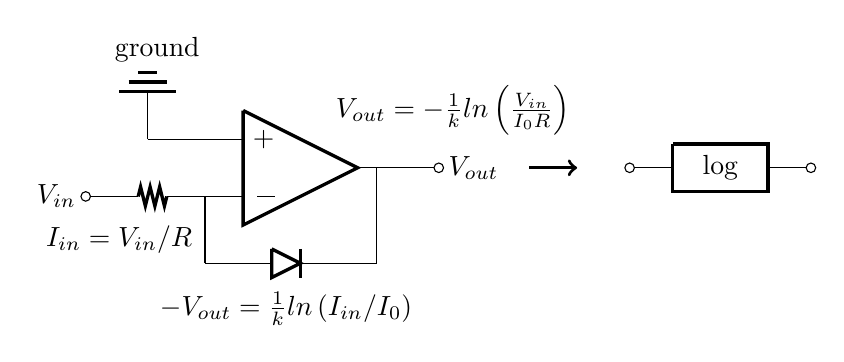
\begin{tikzpicture}[x=0.01\textwidth, y=0.01\textwidth]
\draw [very thick](0,6) -- (12,0) -- (0,-6) -- (0,6);
\draw (-10,3) -- (0,3) node[right]{+};
\draw (-8,-3) -- (0,-3);
\draw (1.5,-3) -- (3.3,-3);
\draw (12,0) -- (20,0);
\draw (20.5,0) circle (0.5) node[right]{$V_{out}$};
\draw (-11,-3) -- (-16,-3);
\draw (-16.5,-3) circle (0.5) node[left]{$V_{in}$};
\draw (-4,-3) -- (-4,-10);
\draw (-4,-10) -- (3,-10);
\draw (6,-10) -- (14,-10) -- (14,0);

%%resistor
\draw [very thick](-11,-3) -- (-10.75, -2) -- (-10.25, -4) -- (-9.75, -2) -- (-9.25,-4) -- (-8.75,-2) -- (-8.25,-4) -- (-8,-3);
%%%
\onslide<2->{
\path (-13,-5) node[below] {$I_{in} = V_{in}/R$};
}
%%%
\draw [very thick](3,-8.5) -- (3,-11.5) -- (6,-10) -- (3,-8.5);
\draw [very thick](6,-8.5) -- (6,-11.5);
%%%%
\onslide<3->{
\path (4.5,-12) node[below]{$- V_{out} = \frac{1}{k} \text{ln} \left( I_{in}/ I_{0}\right)$};
}
%%%
%%ground
\draw (-10,3) -- (-10, 8);
\draw [very thick](-13,8) -- (-7,8);
\draw [very thick](-12,9) -- (-8,9);
\draw [very thick](-11,10) -- (-9,10) node[above]{ground}; 
%%%result
\onslide<4->{
\path (22,6) node{\alert{$V_{out} = - \frac{1}{k} \text{ln} \left( \frac{V_{in}}{ I_{0}R}\right)$}};
}
%%abstraction
\onslide<5->{
\draw [->][very thick] (30,0) -- (35,0);
\draw (40.5,0) circle (0.5);
\draw (41,0) -- (45,0);
\draw [very thick](45,2.5)--(45,-2.5)--(55,-2.5)--(55,2.5)--(45,2.5);
\draw (55,0) -- (59,0);
\draw (59.5,0) circle (0.5);
\path (50,0) node{log};
}
\end{tikzpicture}
%%%%%
%%%%%
\end{frame}

%%%%
\begin{frame}{Differential operator}
%%%%
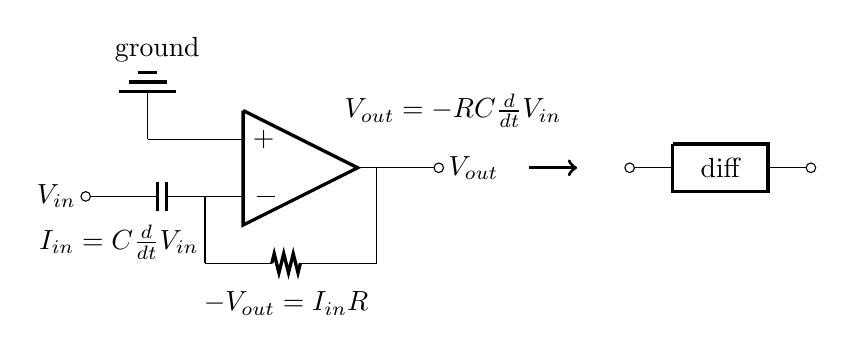
\begin{tikzpicture}[x=0.01\textwidth, y=0.01\textwidth]
\draw [very thick](0,6) -- (12,0) -- (0,-6) -- (0,6);
\draw (-10,3) -- (0,3) node[right]{+};
\draw (-8,-3) -- (0,-3);
\draw (1.5,-3) -- (3.3,-3);
\draw (12,0) -- (20,0);
\draw (20.5,0) circle (0.5) node[right]{$V_{out}$};
\draw (-11,-3) -- (-16,-3);
\draw (-16.5,-3) circle (0.5) node[left]{$V_{in}$};
\draw (-4,-3) -- (-4,-10);
\draw (-4,-10) -- (3,-10);
\draw (6,-10) -- (14,-10) -- (14,0);

%%resistor
\draw (-11,-3)--(-9,-3);
\draw [very thick](-9, -1.5) --(-9,-4.5); 
\draw [very thick](-8,-1.5) -- (-8,-4.5);
%%%
\onslide<2->{
\path (-13,-5) node[below] {$ I_{in} = C \frac{d}{dt}V_{in} $};
}
%%%
\draw [very thick](3,-10) -- (3.25, -9) -- (3.75, -11) -- (4.25, -9) -- (4.75,-11) -- (5.25,-9) -- (5.75,-11) -- (6,-10);
%%%%
\onslide<3->{
\path (4.5,-12) node[below]{$- V_{out} = I_{in} R$};
}
%%%
%%ground
\draw (-10,3) -- (-10, 8);
\draw [very thick](-13,8) -- (-7,8);
\draw [very thick](-12,9) -- (-8,9);
\draw [very thick](-11,10) -- (-9,10) node[above]{ground}; 
%%%result
\onslide<4->{
\path (22,6) node{\alert{$V_{out} = - RC \frac{d}{dt} V_{in} $}};
}
%%abstraction
\onslide<5->{
\draw [->][very thick] (30,0) -- (35,0);
\draw (40.5,0) circle (0.5);
\draw (41,0) -- (45,0);
\draw [very thick](45,2.5)--(45,-2.5)--(55,-2.5)--(55,2.5)--(45,2.5);
\draw (55,0) -- (59,0);
\draw (59.5,0) circle (0.5);
\path (50,0) node{diff};
}
\end{tikzpicture}
%%%%%
\end{frame}

%%%%
\begin{frame}{Integral operator}
%%%%
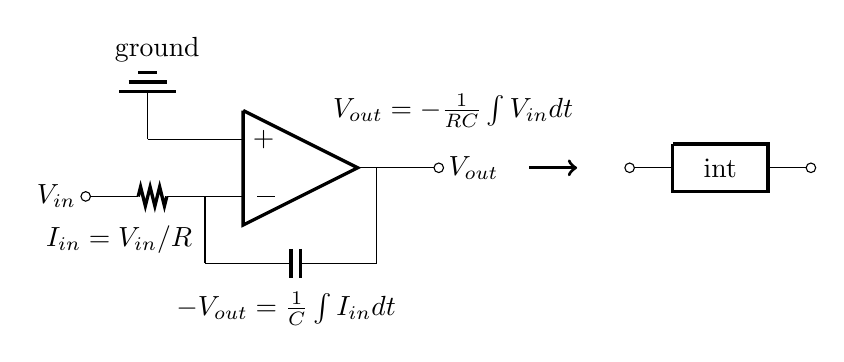
\begin{tikzpicture}[x=0.01\textwidth, y=0.01\textwidth]
\draw [very thick](0,6) -- (12,0) -- (0,-6) -- (0,6);
\draw (-10,3) -- (0,3) node[right]{+};
\draw (-8,-3) -- (0,-3);
\draw (1.5,-3) -- (3.3,-3);
\draw (12,0) -- (20,0);
\draw (20.5,0) circle (0.5) node[right]{$V_{out}$};
\draw (-11,-3) -- (-16,-3);
\draw (-16.5,-3) circle (0.5) node[left]{$V_{in}$};
\draw (-4,-3) -- (-4,-10);
\draw (-4,-10) -- (3,-10);
\draw (6,-10) -- (14,-10) -- (14,0);

%%resistor
\draw [very thick](-11,-3) -- (-10.75, -2) -- (-10.25, -4) -- (-9.75, -2) -- (-9.25,-4) -- (-8.75,-2) -- (-8.25,-4) -- (-8,-3);
%%%
\onslide<2->{
\path (-13,-5) node[below] {$I_{in} = V_{in}/R$};
}
%%%
\draw (5,-10) -- (3,-10);
\draw [very thick](5,-8.5) -- (5,-11.5);
\draw [very thick](6,-8.5) -- (6,-11.5);
%%%%
\onslide<3->{
\path (4.5,-12) node[below]{$- V_{out} = \frac{1}{C} \int I_{in} dt$};
}
%%%
%%ground
\draw (-10,3) -- (-10, 8);
\draw [very thick](-13,8) -- (-7,8);
\draw [very thick](-12,9) -- (-8,9);
\draw [very thick](-11,10) -- (-9,10) node[above]{ground}; 
%%%result
\onslide<4->{
\path (22,6) node{\alert{$V_{out} = - \frac{1}{RC} \int V_{in} dt$}};
}
%%abstraction
\onslide<5->{
\draw [->][very thick] (30,0) -- (35,0);
\draw (40.5,0) circle (0.5);
\draw (41,0) -- (45,0);
\draw [very thick](45,2.5)--(45,-2.5)--(55,-2.5)--(55,2.5)--(45,2.5);
\draw (55,0) -- (59,0);
\draw (59.5,0) circle (0.5);
\path (50,0) node{int};
}
\end{tikzpicture}
%%%%%
\end{frame}

%%
\subsection{Multi - Signal Operator}
%%%
%%%
\begin{frame}{Addition operator}
%%%%
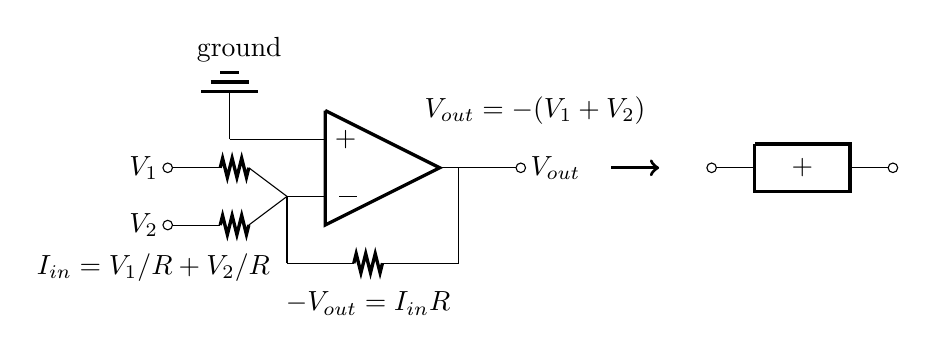
\begin{tikzpicture}[x=0.01\textwidth, y=0.01\textwidth]
\draw [very thick](0,6) -- (12,0) -- (0,-6) -- (0,6);
\draw (-10,3) -- (0,3) node[right]{+};
\draw (-4,-3) -- (0,-3);
\draw (1.5,-3) -- (3.3,-3);
\draw (12,0) -- (20,0);
\draw (20.5,0) circle (0.5) node[right]{$V_{out}$};
%%%%
\draw (-11,0) -- (-16,0);
\draw (-16.5,0) circle (0.5) node[left]{$V_{1}$};
\draw (-11,-6) -- (-16,-6);
\draw (-16.5,-6) circle (0.5) node[left]{$V_2$};
%%%%
\draw (-4,-3) -- (-4,-10);
\draw (-4,-10) -- (3,-10);
\draw (6,-10) -- (14,-10) -- (14,0);

%%resistor
\draw [very thick](-11,0) -- (-10.75, 1) -- (-10.25, -1) -- (-9.75, 1) -- (-9.25,-1) -- (-8.75,1) -- (-8.25,-1) -- (-8,0);
\draw (-8,0) -- (-4,-3);
%%
\draw [very thick](-11,-6) -- (-10.75, -5) -- (-10.25, -7) -- (-9.75, -5) -- (-9.25,-7) -- (-8.75,-5) -- (-8.25,-7) -- (-8,-6);
\draw (-8,-6) -- (-4,-3);
%%%
\onslide<2->{
\path (-18,-8) node[below] {$I_{in} = V_1 /R + V_2 /R$};
}
%%%
\draw [very thick](3,-10) -- (3.25, -9) -- (3.75, -11) -- (4.25, -9) -- (4.75,-11) -- (5.25,-9) -- (5.75,-11) -- (6,-10);
%%%%
\onslide<3->{
\path (4.5,-12) node[below]{$- V_{out} = I_{in} R$};
}
%%%
%%ground
\draw (-10,3) -- (-10, 8);
\draw [very thick](-13,8) -- (-7,8);
\draw [very thick](-12,9) -- (-8,9);
\draw [very thick](-11,10) -- (-9,10) node[above]{ground}; 
%%%result
\onslide<4->{
\path (22,6) node{\alert{$V_{out} = - ( V_1 + V_2 )$}};
}
%%abstraction
\onslide<5->{
\draw [->][very thick] (30,0) -- (35,0);
\draw (40.5,0) circle (0.5);
\draw (41,0) -- (45,0);
\draw [very thick](45,2.5)--(45,-2.5)--(55,-2.5)--(55,2.5)--(45,2.5);
\draw (55,0) -- (59,0);
\draw (59.5,0) circle (0.5);
\path (50,0) node{+};
}
\end{tikzpicture}
%%%%%
\end{frame}
%%%
%%%
\begin{frame}{Multiplication operator}
%%%%
\onslide<2->{
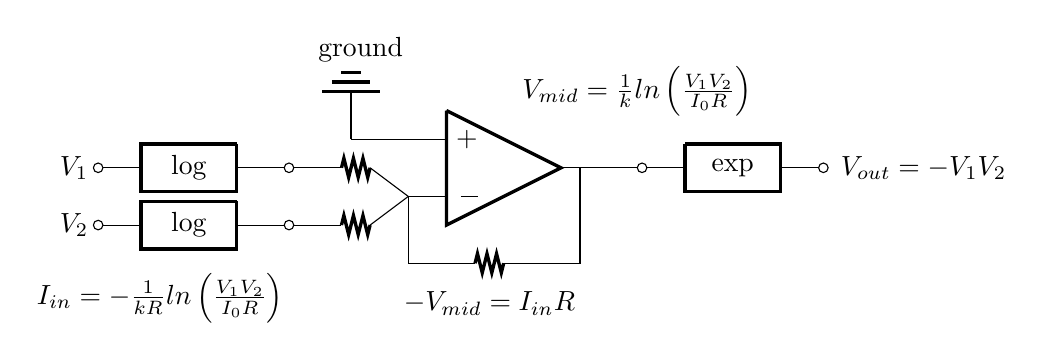
\begin{tikzpicture}[x=0.01\textwidth, y=0.01\textwidth]
\draw [very thick](0,6) -- (12,0) -- (0,-6) -- (0,6);
\draw (-10,3) -- (0,3) node[right]{+};
\draw (-4,-3) -- (0,-3);
\draw (1.5,-3) -- (3.3,-3);
\draw (12,0) -- (20,0);
\draw (20.5,0) circle (0.5);
%%%%
\draw (-11,0) -- (-16,0);
\draw (-16.5,0) circle (0.5);
\draw (-11,-6) -- (-16,-6);
\draw (-16.5,-6) circle (0.5);
%%%%
\draw (-4,-3) -- (-4,-10);
\draw (-4,-10) -- (3,-10);
\draw (6,-10) -- (14,-10) -- (14,0);

%%resistor
\draw [very thick](-11,0) -- (-10.75, 1) -- (-10.25, -1) -- (-9.75, 1) -- (-9.25,-1) -- (-8.75,1) -- (-8.25,-1) -- (-8,0);
\draw (-8,0) -- (-4,-3);
\draw (-17,0) -- (-22,0);
\draw [very thick] (-22,2.5) -- (-22,-2.5) -- (-32,-2.5) -- (-32,2.5) -- (-22,2.5);
\draw (-32,0) -- (-36,0);
\draw (-36.5,0) circle (0.5) node[left]{$V_1$};
\path (-27,0) node{log};
%%
\draw [very thick](-11,-6) -- (-10.75, -5) -- (-10.25, -7) -- (-9.75, -5) -- (-9.25,-7) -- (-8.75,-5) -- (-8.25,-7) -- (-8,-6);
\draw (-8,-6) -- (-4,-3);
\draw(-17,-6) -- (-22,-6);
\draw [very thick] (-22, -3.5) -- (-22,-8.5) -- (-32,-8.5) -- (-32,-3.5) -- (-22,-3.5);
\draw (-32,-6) -- (-36,-6);
\draw (-36.5, -6) circle (0.5) node[left]{$V_2$};
\path (-27,-6) node{log};
%%%
\onslide<3->{
\path (-30,-10) node[below] {$I_{in} = - \frac{1}{kR} \text{ln} \left( \frac{V_1 V_2}{I_0 R} \right)$};
}
%%%
\draw [very thick](3,-10) -- (3.25, -9) -- (3.75, -11) -- (4.25, -9) -- (4.75,-11) -- (5.25,-9) -- (5.75,-11) -- (6,-10);
%%%%
\onslide<4->{
\path (4.5,-12) node[below]{$- V_{mid} = I_{in} R$};
}
%%%
%%ground
\draw (-10,3) -- (-10, 8);
\draw [very thick](-13,8) -- (-7,8);
\draw [very thick](-12,9) -- (-8,9);
\draw [very thick](-11,10) -- (-9,10) node[above]{ground}; 
%%%result
\onslide<5->{
\path (20,8) node{$V_{mid} =  \frac{1}{k} \text{ln} \left( \frac{V_1 V_2}{I_0 R} \right)$};
}
%%abstraction
\onslide<6->{
\draw (21,0) -- (25,0);
\draw [very thick] (25,2.5) -- (25,-2.5) -- (35,-2.5) -- (35,2.5) -- (25,2.5);
\draw (35,0) -- (39,0);
\draw (39.5,0) circle (0.5);
\path (30,0) node{exp};
}
\onslide<7->{
\path (50,0) node{\alert{$V_{out} = - V_1 V_2$}};
}
\end{tikzpicture}
}
%%%%%
%%%%%
\end{frame}

%%Meaning of Op signal
\section{Meaning of Operating Signal}

\subsection{Operating Signal and Modern Human Society}

\begin{frame}{From Amplifier to Information Revolution}
As amplifiers have developed from \alert{vacuum tube} $\rightarrow$ \alert{transistor} $\rightarrow$ \alert{integrated circuit embedded amplifier}, combined with switching logic circuit, became modern processor which enable the \alert{Information Revolution}
\onslide<2->{
\begin{center}
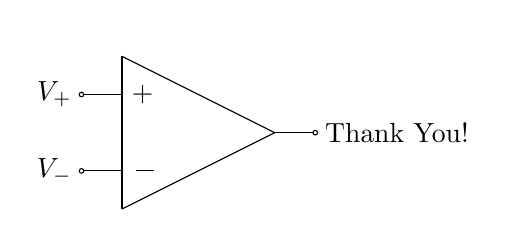
\begin{tikzpicture}[x=0.02\textwidth, y=0.02\textwidth]
%positioning
\path (0,5.5)--(0,5);
%%body
\draw[-] [bd] (0,-4)--(0,4);
\draw[-] [bd] (0,4)--(8,0);
\draw[-] [bd] (0,-4)--(8,0);
%%wire
\draw[-] [bd] (-2,2)--(0,2); 
\path (0,2) node[right]{+};
\draw[-] [bd] (-2,-2)--(0,-2); 
\draw (0.75,-2) -- (1.65,-2) ;
\draw[-] [bd] (8,0)--(10,0);
%%node
\draw (-2.12,-2) circle (0.12) node[left] {$V_-$};
\draw (-2.12,2) circle (0.12) node[left]{$V_+$};
\draw (10.12,0) circle (0.12) node[right]{\alert{Thank You!}};
\end{tikzpicture}
\end{center}
}
\end{frame}

\end{document}
